\section*{\'Etat de l'art}
\addcontentsline{toc}{section}{\'Etat de l'art}
Nous avons recherché plusieurs projet proche de la desserte robotisée.

\subsection*{Robot Numéro 1 de Firstclass Robotics}
Ce projet est très proche de notre desserte d'un point de vue
fonctionnel. En effet, il est prévu pour servir lors de reception. il
est déjà en service et peut être loué au près de First Class
Robotique.

\begin{figure}[h]
\begin{center}
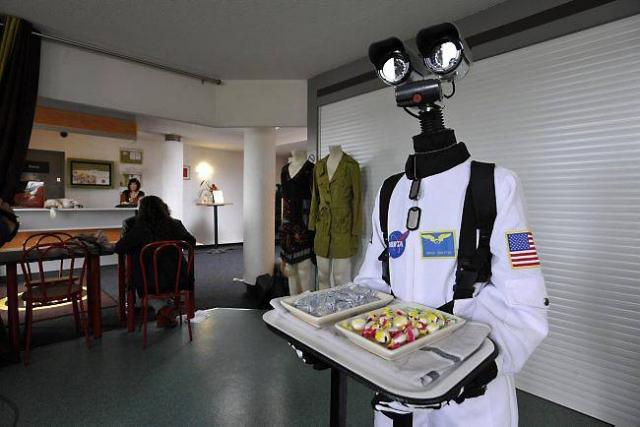
\includegraphics[scale=0.55]{Images/robot_n1.jpg}
\caption{robot Numéro 1}
\label{robot Numéro 1}
\end{center}
\end{figure} 

Ce robot à été conçu par Bernard MARTI, qui à notamment été professeur
de robotique à l'INSA de Lyon. Ce robot à clairement été conçu d'un
point de vue industriel et dans une optique de faire un robot à bas
coût. Il coute 15000 euros.  A noter que le concepteur est assez
accessible est peut être contacté par mail ou par téléphone.

Site internet: \url{http://firstclass.robotics.online.fr/}

\subsubsection*{Caractéristiques}
le robot fait 1m55, à une autonomie de 12h, et utilise un système de
vision basé à la fois sur des capteur infrarouge et et des capteurs
ultrasons et permettant une vision à 12m.

Le robot ce caractèrise aussi par une absence de communication avec
une base, permettant de le rendre insensible à tout pratage
informatique. il est complètement autonome et ne necessite pas de
cartographie. Bernard MARTI parle d'ailleur de programmation
insectoïde et réduite au minimum.

A noté qu'une version "plus" existe également, plus axée assistance.

\subsubsection*{Contexte}

Une différence majeure de ce robot par rapport à notre projet est que ce robot n'essaye pas d'imiter un serveur, mais se presente plutôt comme un robot d'aide au serveur. Le concepteur du robot indique par ailleurs que le robot à été plutôt bien accueilli par les professionel qui officiait a ses côtés. 

\subsection*{Care O Bot}

Le care O bot s'écarte un peu de notre projet mais reste à étudier. Il
s'agit d'un robot d'aide à la personne, équipé d'un bras articulé et
d'un plateau. il est construit par Fraunhofer, une entreprise
allemande.

\subsubsection*{Caractéristiques}

\begin{figure}[h]
\begin{center}
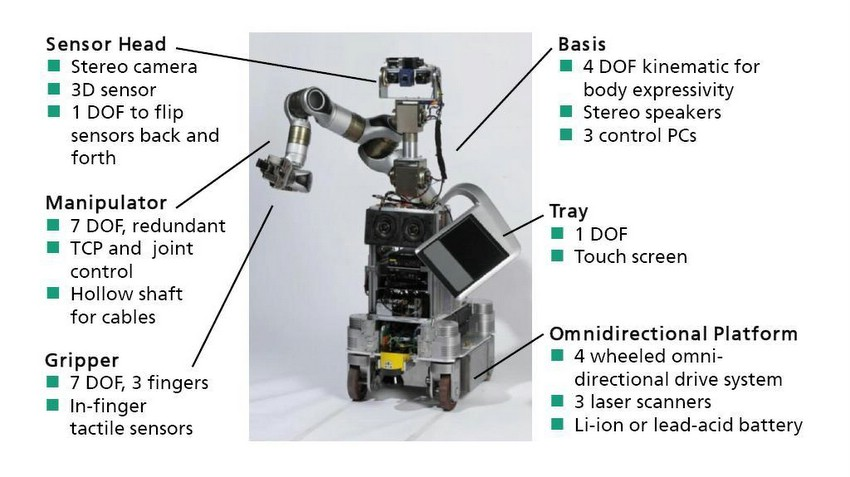
\includegraphics[scale=0.55]{Images/cob3-hardware.jpg}
\caption{caractéristique du careObot3}
\label{caractéristique du careObot3}
\end{center}
\end{figure}

Le robot roule d'une manière lente et fluide. Il utilise des caméras et des capteur de profondeurs pour se reperer, ainsi qu'un système de cartographie. Son bras possède 7 degré de liberté. pour intéragir, il dispose d'une tablette tactile sur son plateau ainsi que d'une reconnaissance faciale et auditive. Il dispose aussi d'haut parleur pour communiquer.

\subsubsection*{Contexte}

Ce robot évolue dans un contexte très différents de notre desserte. Il se trouve chez des particuliers ou dans des maisons de retraites. Il n'a donc pas les mêmes contraintes en terme de gestion de foule et de déplacement. En revanche il peut-être très interessant d'étudier sa façon de servir et de s'approcher des humains.

site internet du constructeur:\\
\url{http://www.care-o-bot.de/de/care-o-bot-3.html}

\newpage

\subsection*{Dalu Robot}

Dalu Robot n'est pas un robot, mais un restaurant chinois qui utilise plusieurs robot pour servir leurs clients. Ces robot sont assez rudimentaires en soi, puisqu'ils suivent une ligne blanche au sol qui fait le tour de la pièce et s'arretes losrqu'un humain s'arrête. Néanmoins, ils sont conçu pour évoluer en mileu humain et leur design peut-être interessant à étudier.

\begin{figure}[h]
\begin{center}
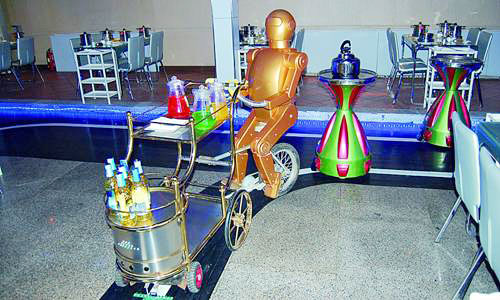
\includegraphics[scale=0.55]{Images/dalu-robot-1.jpg}
\caption{exemple de robot chez Dalu Robot}
\label{exemple de robot chez Dalu Robot}
\end{center}
\end{figure}

\subsection*{Projet MOSAIC}

Le projet MOSAIC est un projet collaboratif européen visant à créer
des robots de service a partir d'une base commune déjà développée:

\begin{itemize}
\item Robot Room service / version Hôtel
\item Room service / version domestique et yacht
\item Robot bar
\item Robot "maître d'hôtel" pour les restaurants haut de gamme
\item Robot coursier d’entreprise
\end{itemize}

Ils travaillent donc sur un projet relativement proche du nôtre bien
que l'approche soit plus généraliste.

\begin{figure}[h]
\begin{center}
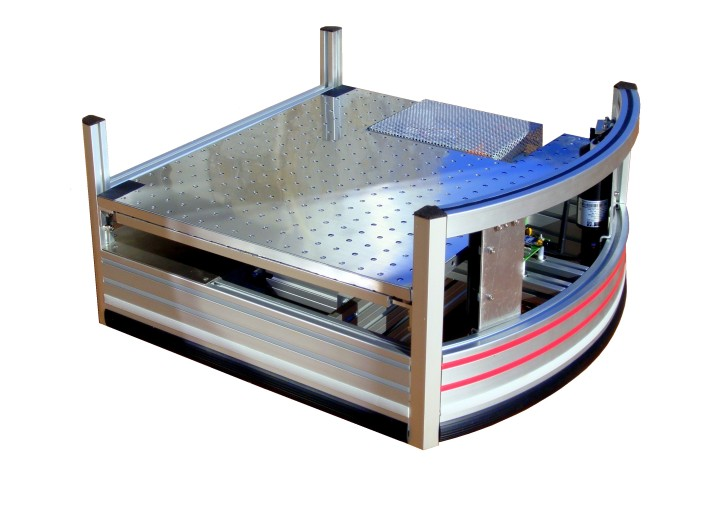
\includegraphics[scale=0.55]{Images/robot_mosaic}
\caption{Prototype du robot existant}
\label{Prototype du robot existant}
\end{center}
\end{figure} 

\subsubsection*{Caractéristiques}
\begin{itemize}
\item Ce robot est propulsé par deux roues motrice et deux roues libres.
\item Les moteurs sont des moteurs pas à pas d'une puissance de $450W$
  ce qui lui permet de se déplacer à une vitesse maximale de $0.84m/s$
  avec une accéleration maximale de $1m/s^2$ et un arrêt d'urgence à
  $-1.6m/s^2$.
\item Le chassis est en aluminium et en acier.
\item La batterie à une capacité de 480W/h (batterie au plomb).
\item Carte wifi pour la communication
\end{itemize}

le site internet contient pas mal d'information et des vidéo de présentation:\\
\url{http://www.bf-io.com/robots_FR.html}

\subsection*{Laksmi-Do} 
Il s'agit d'un table robotisée télécommandée sur deux roues uniquement
(elle utilise le principe du Sigway).

\begin{figure}[h]
\begin{center}
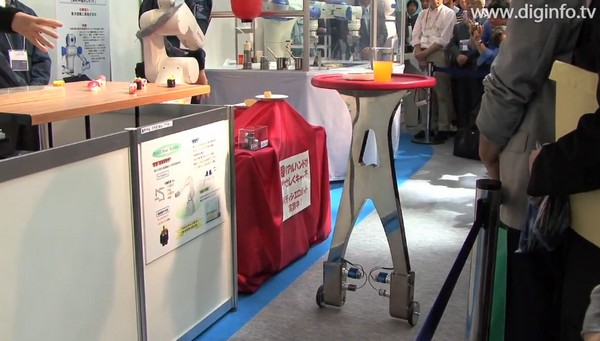
\includegraphics[scale=0.55]{Images/laksmido_table.jpg}
\caption{Table robotisée télécommandée}
\label{Table robotisée télécommandée}
\end{center}
\end{figure} 

Les caractéristiques exactes de la tables sont difficiles à trouver
car le site du projet est en japonais. cependant nous savons que les
concepteur de cette table travaille à la rendre autonome, à lui faire
reconnaitre la voix, et compte la rendre capable de porter une charge
utile de $50Kg$.

site internet:\url{http://www.laksmido.com/robotics.html}
